\documentclass[]{article}
\usepackage{lmodern}
\usepackage[compact]{titlesec}
\usepackage{amssymb,amsmath}
\usepackage{ifxetex,ifluatex}
\usepackage{fixltx2e} % provides \textsubscript
\ifnum 0\ifxetex 1\fi\ifluatex 1\fi=0 % if pdftex
  \usepackage[T1]{fontenc}
  \usepackage[utf8]{inputenc}
\else % if luatex or xelatex
  \ifxetex
    \usepackage{mathspec}
  \else
    \usepackage{fontspec}
  \fi
  \defaultfontfeatures{Ligatures=TeX,Scale=MatchLowercase}
\fi
% use upquote if available, for straight quotes in verbatim environments
\IfFileExists{upquote.sty}{\usepackage{upquote}}{}
% use microtype if available
\IfFileExists{microtype.sty}{%
\usepackage{microtype}
\UseMicrotypeSet[protrusion]{basicmath} % disable protrusion for tt fonts
}{}
\usepackage[margin=1in]{geometry}
\usepackage{hyperref}
\hypersetup{unicode=true,
            pdftitle={Solo 3: Campaign Response Modeling},
            pdfauthor={Darryl Buswell},
            pdfborder={0 0 0},
            breaklinks=true}
\urlstyle{same}  % don't use monospace font for urls
\usepackage{longtable,booktabs}
\usepackage{graphicx,grffile}
\makeatletter
\def\maxwidth{\ifdim\Gin@nat@width>\linewidth\linewidth\else\Gin@nat@width\fi}
\def\maxheight{\ifdim\Gin@nat@height>\textheight\textheight\else\Gin@nat@height\fi}
\makeatother
% Scale images if necessary, so that they will not overflow the page
% margins by default, and it is still possible to overwrite the defaults
% using explicit options in \includegraphics[width, height, ...]{}
\setkeys{Gin}{width=\maxwidth,height=\maxheight,keepaspectratio}
\IfFileExists{parskip.sty}{%
\usepackage{parskip}
}{% else
\setlength{\parindent}{0pt}
\setlength{\parskip}{6pt plus 2pt minus 1pt}
}
\setlength{\emergencystretch}{3em}  % prevent overfull lines
\providecommand{\tightlist}{%
  \setlength{\itemsep}{0pt}\setlength{\parskip}{0pt}}
\setcounter{secnumdepth}{0}
% Redefines (sub)paragraphs to behave more like sections
\ifx\paragraph\undefined\else
\let\oldparagraph\paragraph
\renewcommand{\paragraph}[1]{\oldparagraph{#1}\mbox{}}
\fi
\ifx\subparagraph\undefined\else
\let\oldsubparagraph\subparagraph
\renewcommand{\subparagraph}[1]{\oldsubparagraph{#1}\mbox{}}
\fi

%%% Use protect on footnotes to avoid problems with footnotes in titles
\let\rmarkdownfootnote\footnote%
\def\footnote{\protect\rmarkdownfootnote}

%%% Change title format to be more compact
\usepackage{titling}

% Create subtitle command for use in maketitle
\newcommand{\subtitle}[1]{
  \posttitle{
    \begin{center}\large#1\end{center}
    }
}

\setlength{\droptitle}{-2em}
  \title{Solo 3: Campaign Response Modeling}
  \pretitle{\vspace{\droptitle}\centering\huge}
  \posttitle{\par}
\subtitle{MSPA PREDICT 450-DL-55 LEC}
  \author{Darryl Buswell}
  \preauthor{\centering\large\emph}
  \postauthor{\par}
  \date{}
  \predate{}\postdate{}

\begin{document}
\maketitle

\section{1 Introduction}\label{introduction}

This document presents the results of the third assignment for the
Masters of Science in Predictive Analytics course: PREDICT 450. This
assessment required the student to develop a predictive model in order
to identify customers that are likely to respond to a mailing campaign,
and once identified, estimate the net profit that may result from
targeting those customers as part of a new mailing campaign.

For this assessment, we leverage XYZ's database of customers which
contains a large number of variables relating to sales and campaign
results. We use this data to first assess which variables have the
greatest `importance' in determining both the chance of response to a
mailing campaign as well as the likely spend of each customer. We then
use this reduced dataset to fit three classification models to predict
chance of response, and three regression models to predict likely spend.
Optimal models are selected and subsequently used in order to estimate
the expected net revenue from conducting a new targeted mailing
campaign, accounting for the cost of mailing each customer.

\section{2 Data}\label{data}

The dataset used for this assessment is based on XYZ's database of
customers. It includes 30,779 records and 554 features of customer data.
The features capture customer sales, results from previous mailing
campaigns, and Experian properties which provide additional insights
about each customer. The features are broken up into 345 character, 48
integer and 161 numeric variable types.

Due to the scale of data, we conducted a subjective assessment of
variable relevance prior to employing any pre-processing or modelling
routines. We did this by assessing the descriptions for variables
contained within the provided data dictionary and grading each by its
perceived ability to predict both the chance of response and likely
spend. This resulted in 227 variables being graded as having a `low'
relevance, which were subsequently excluded from the dataset. Note that
a summary data file of each variable grade is available on request. The
remaining variables can be broken up into 119 character, 48 integer and
160 numeric variable types.

From an initial look at the data, we noted that the compiled R data
frame fails to distinguish between numeric and factor variables. As
such, prior to performing any data exploration, we converted all
character class variables to factor type and retained all other
variables as numeric type. We then manually converted all `ANY\_MAIL\_x'
and `RESPONSEx' variables to factor type, since these variables
contained no character based observations yet were observed to be
categorical in nature.

\section{3 Data Exploration}\label{data-exploration}

A number of exploration routines were conducted. These routines allowed
us to gain an understanding of potential data limitations, including
identifying variables which have missing observations, outlier
observations, or those variables which may benefit from transformation.

\subsection{3.1 Univariate Data
Analysis}\label{univariate-data-analysis}

As part of the univariate data analysis, summary statistics for all of
the 160 retained numeric variables were calculated and observed. The
majority of numeric variables do not suffer from missing values.
However, many variables have a minimum value of zero, suggesting
zero-inflated data. Histogram and box plots were also generated and
reviewed for a large subset of numeric variables, with total amount
spent (TOTAMT) selected for further discussion below. Note that zero
value observations were removed prior to generating each plot.

\paragraph{Figure 3.1.1 Histogram and Boxplot:
TOTAMT}\label{figure-3.1.1-histogram-and-boxplot-totamt}

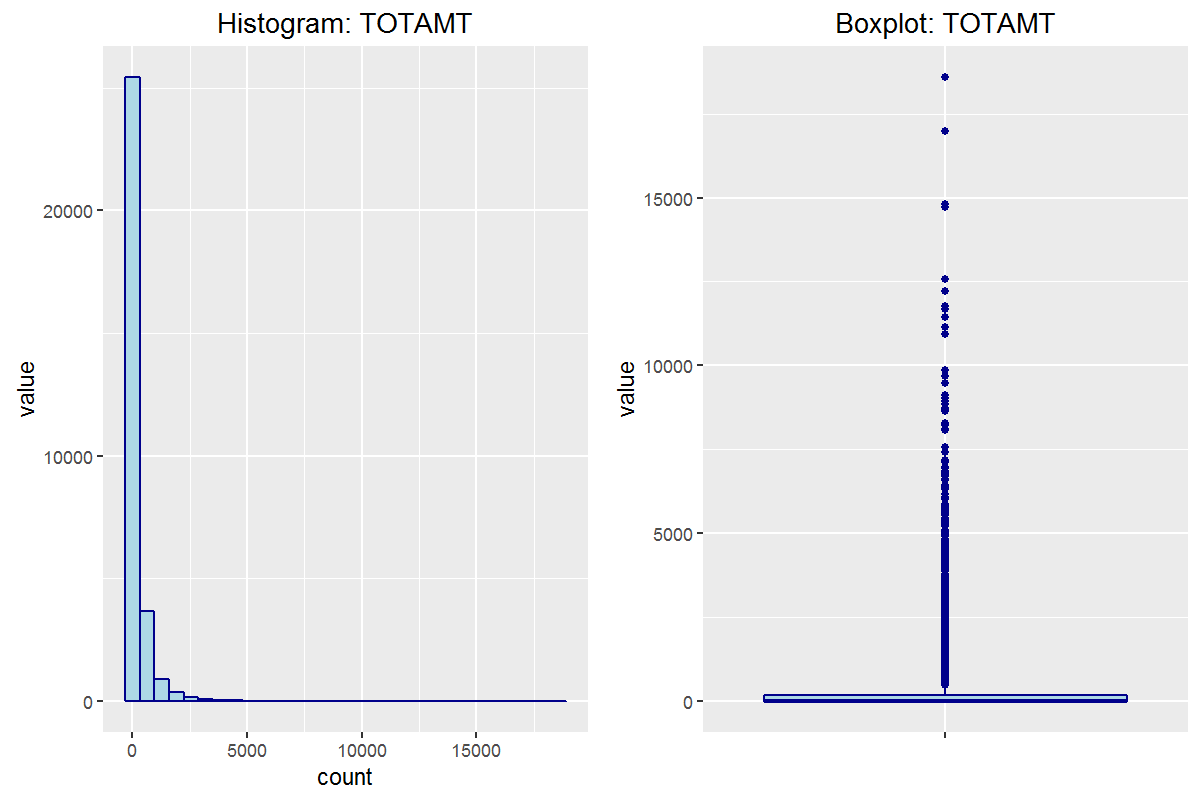
\includegraphics[height=3.33333in]{images/expl_num_TOTAMT.png}

We immediately noticed that the variable suffers from a heavy positive
skew, which is in-fact a common attribute over the majority of numeric
variables. The result is a number of observations which could be classed
as outliers.

\subsection{3.2 Bivariate Data Analysis}\label{bivariate-data-analysis}

Since we intend on building a prediction model to determine both the
chance of response to a mailing campaign (RESPONSE16) and the likely
spend of each customer (TOTAMT16), we have an interest in identifying
variables which have explanatory power over these two variables. As
such, we calculated and reviewed the Pearson correlation coefficient for
all numeric variables against our numeric response variable, TOTAMT16.
Correlations for the 10 most correlated numeric variables against
TOTAMT16 are shown in the table below.

\subsubsection{Table 3.2.1 Correlations vs.~TOTAMT16 (Top 10
Correlations)}\label{table-3.2.1-correlations-vs.totamt16-top-10-correlations}

\begin{longtable}[]{@{}ll@{}}
\toprule
variable & correl coeff\tabularnewline
\midrule
\endhead
YTD\_SALES\_2009 & 0.3723\tabularnewline
YTD\_TRANSACTIONS\_2009 & 0.2938\tabularnewline
LTD\_SALES & 0.2218\tabularnewline
LTD\_TRANSACTIONS & 0.2067\tabularnewline
PRE2009\_TRANSACTIONS & 0.1587\tabularnewline
PRE2009\_SALES & 0.1445\tabularnewline
TOTAL\_MAIL\_13 & 0.1182\tabularnewline
TOTAL\_MAIL\_14 & 0.1178\tabularnewline
TOTAL\_MAIL\_15 & 0.1178\tabularnewline
SUM\_MAIL\_12 & 0.1158\tabularnewline
\bottomrule
\end{longtable}

None of the variables have reported a strong correlation with TOTAMT16,
with the greatest absolute correlation being reported by total sales
through to 2009 (YTD\_SALES\_2009) and total transactions through to
2009 (YTD\_TRANSACTIONS\_2009) at 0.37 and 0.29, respectively. Finally,
we used bar plots to explore the relationship between the categorical
response variable (RESPONSE16) and each numeric variable. Two of these
plots have been selected for further discussion below.

\paragraph{Figure 3.2.1 Boxplot: RESPONSE16 vs.~TOTAMT /
QTY}\label{figure-3.2.1-boxplot-response16-vs.totamt-qty}

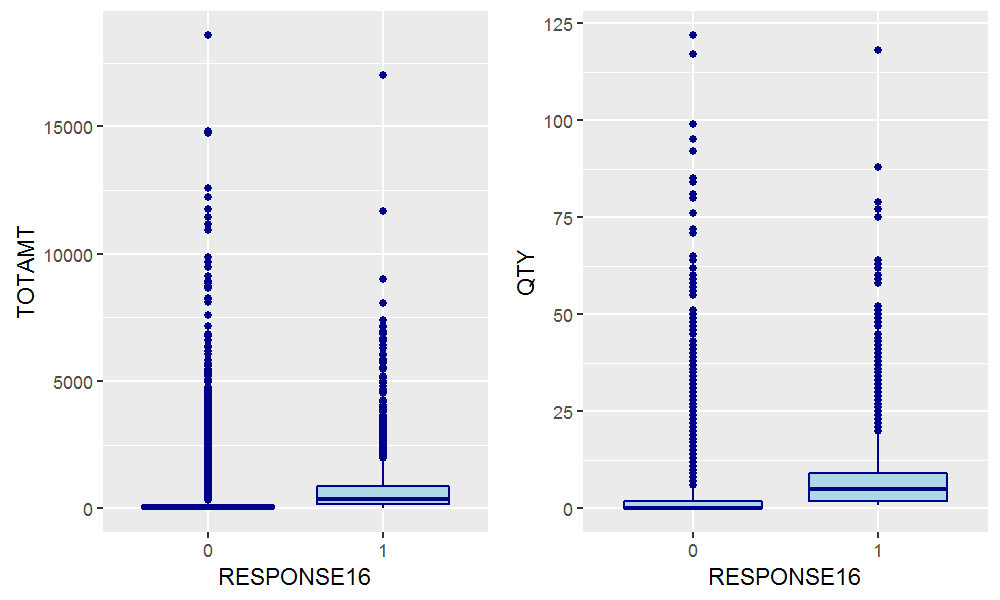
\includegraphics[height=3.33333in]{images/expl_boxcomp_1.png}

We can see that there are indeed recognizable differences in both the
mean and distribution of a number of numeric variables depending on
whether they are associated with a positive or negative response to an
advertising mailing campaign.

\section{4 Data Pre-processing}\label{data-pre-processing}

As part of the data pre-processing routine, we first focused on imputing
data for missing observations (\textasciitilde{}11\% of the dataset).
This was initially attempted using the rfImpute function from the Random
Forest package in R, however processing time eliminated this as a viable
option. Instead, we looped over each variable and imputed observations
for numeric variables with the variables' median value, and at the same
time, imputed observations for character variables with the variables'
most common value. Those variables which required imputation were copied
and renamed to include the suffix '\_IMP' while the original
(non-imputed) equivalent was removed from the dataset. Note that while
89 of the retained categorical variables were identified as having
missing values, only one of the retained numeric variables, ECHVPCT, was
identified as having missing values.

We then looked towards dealing with outlier observations for numeric
variables. In many cases, the task of identifying outlier observations
can be a subjective practice. As such, for this assessment, we took a
statistical approach and targeted those observations which fell outside
the 1st and 99th percentile range. Observations which met these criteria
were replaced using the squish function as part of the scales package in
R, effectively resulting in a newly created set of trimmed variables.
Trimmed variables added to the dataset and can be recognized by the
suffix '\_T99'.

Finally, we looked towards creating dummies for each of the retained
factor variables. Our first preference was to convert all factor
variables to dummies, however we noted that many had a high level count
and a number of levels with relatively low occurrence. As such, we
elected to create dummies for only those factors which had 10 or less
levels. Dummy variables were named to include the prefix `DUM\_', along
with a suffix to represent the factor level. Note that k-1 dummies were
created, where k is the original number of levels for each variable.
This resulted in the creation of 351 dummies.

\section{5 Variable Importance}\label{variable-importance}

The data processing routine produced a data frame of 586 numeric
variables. With such a large dataset, it was clear that any subsequent
model estimation would benefit from a further reduction in variable
count. To achieve this, we leveraged the varImp function as part of the
caret package in R to calculate the variable importance according to
both response variables. In both cases, variable importance was
calculated by fitting a Random Forest model, with `importance' measured
by the mean decrease in node impurity. Bar plots of the 20 most
important variables for both response variables are below.

\paragraph{Figure 5.1 Variable Importance:
RESPONSE16}\label{figure-5.1-variable-importance-response16}

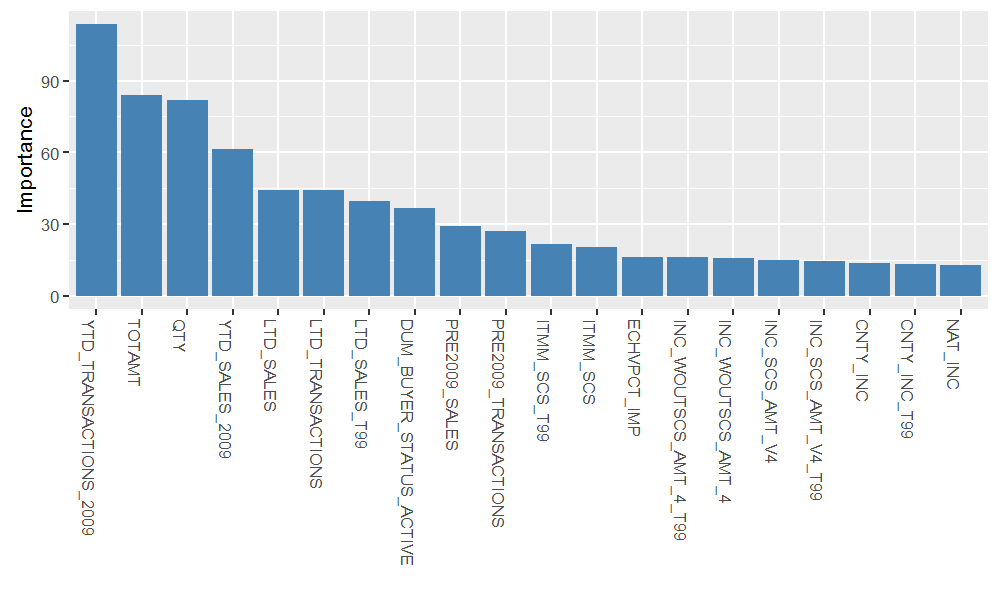
\includegraphics[height=3.02083in]{images/varimp_response16.png}

\paragraph{Figure 5.2 Variable Importance:
TOTAMT16}\label{figure-5.2-variable-importance-totamt16}

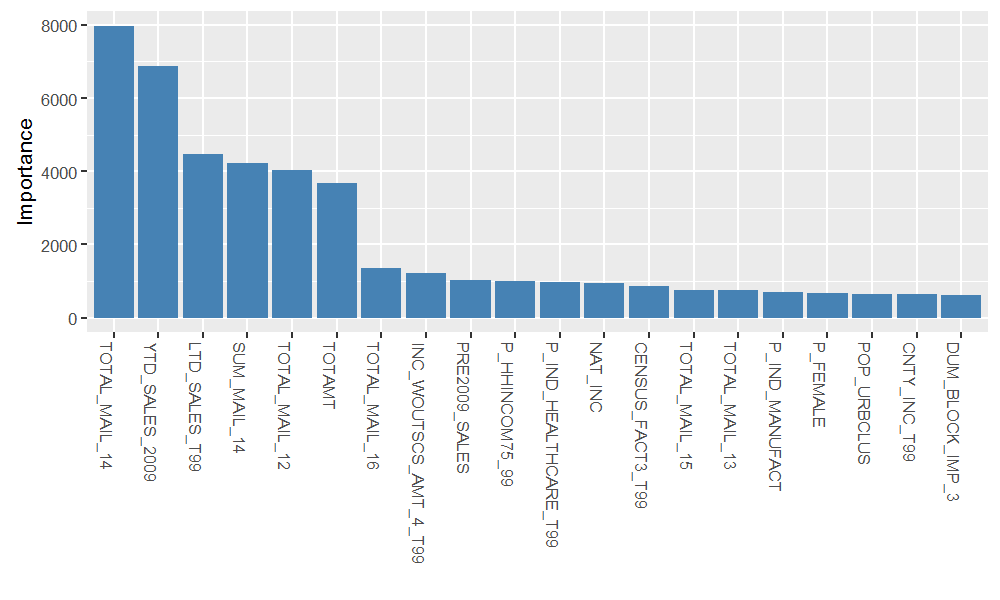
\includegraphics[height=3.02083in]{images/varimp_totamt16.png}

We can see some commonality between variable importance plots, with
TOTAMT, YTD\_SALES\_2009 and PRE2009\_SALES all within the top-10 rank
for both response variables. We also note a fairly quick drop-off in
variable importance beyond the first five variables within both plots.
Based on these results, we elected to pass the top-50 ranked variables
by importance through to our model estimation phase. We believe this
reduction provides a suitable trade-off both in terms of accuracy and
performance.

\section{6 Model Estimation}\label{model-estimation}

\subsection{6.1 Classification Modelling: Chance of
Response}\label{classification-modelling-chance-of-response}

For this assessment, we fit three classification based models in order
to predict the chance a customer will respond to a mailing campaign.
These models include a Naive Bayes, Random Forest and a Lasso and
Elastic-Net Regularized Generalized Linear Model (GLMnet) classifier. In
each case, we leverage the train function as part of the caret package
with a 3-fold cross-validation sampling method, which was applied to a
70\% subset of training data and tested against a 30\% subset. Default
parameters were used for each model.

The in and out-of-sample Receiver Operating Characteristic (ROC) Curves
are shown for each model in Appendix A. The Naive Bayes classifier
managed to deliver an in-sample Area Under the Curve (AUC) of 0.85,
while its out-of-sample AUC was 0.82. Clearly, the classifier has
avoided over-fitting the training data and has managed to maintain
similar classification performance over both the training and test sets.
The Random Forest classifier on the other hand, reported an in-sample
AUC of 1.00 and an out-of-sample AUC of 0.85, which suggests that it
greatly suffers from over-fitting. Finally, the GLMnet classifier
generated an in-sample AUC of 0.87 and out-of-sample AUC of 0.86.

Below we show the out-of-sample confusion matrix for each model.

\paragraph{Table 6.1.1 Confusion Matrix: Classification Model
Comparison}\label{table-6.1.1-confusion-matrix-classification-model-comparison}

\begin{longtable}[]{@{}lllllllllll@{}}
\toprule
Naive Bayes & & & & Random Forest & & & & GLMnet & &\tabularnewline
\midrule
\endhead
& Pred: 0 & Pred: 1 & & & Pred: 0 & Pred: 1 & & & Pred: 0 & Pred:
1\tabularnewline
Actual: 0 & 3503 & 246 & & Actual: 0 & 3992 & 452 & & Actual: 0 & 4004 &
416\tabularnewline
Actual: 1 & 496 & 218 & & Actual: 1 & 7 & 12 & & Actual: 1 & 20 &
38\tabularnewline
\bottomrule
\end{longtable}

We can see that while the Random Forest and GLMnet classifiers were able
to produce similar out-of-sample performance according to their ROC
curves, the Random Forest classifier has done so by providing less true
positive and true negative values. We can confirm this by observing the
performance metrics in the table below, which shows that the GLMnet
classifier was able to obtain a superior true positive rate and true
negative rate.

\paragraph{Table 6.1.2 Performance Metrics: Classification Model
Comparison}\label{table-6.1.2-performance-metrics-classification-model-comparison}

\begin{longtable}[]{@{}llll@{}}
\toprule
& Naive Bayes & Random Forest & GLMnet\tabularnewline
\midrule
\endhead
Accuracy & 0.8337 & 0.8972 & 0.9026\tabularnewline
95\% CI & (0.8225, 0.8446) & (0.8879, 0.9059) & (0.8936,
0.9112)\tabularnewline
Kappa & 0.2793 & 0.0419 & 0.1284\tabularnewline
Sensitivity & 0.4698 & 0.0259 & 0.0837\tabularnewline
Specificity & 0.8760 & 0.9983 & 0.9950\tabularnewline
Pos Pred Value & 0.3053 & 0.6316 & 0.6552\tabularnewline
Neg Pred Value & 0.9344 & 0.8983 & 0.9059\tabularnewline
Prevalence & 0.1040 & 0.1040 & 0.1014\tabularnewline
Detection Rate & 0.0489 & 0.0027 & 0.0085\tabularnewline
Detection Prevalence & 0.1600 & 0.0043 & 0.0130\tabularnewline
Balanced Accuracy & 0.6729 & 0.5121 & 0.5394\tabularnewline
\bottomrule
\end{longtable}

From a view of the performance metrics above, we can see that the GLMnet
model has demonstrated a superior AUC, accuracy, sensitivity and
specificity compared to the other models. As such, we have elected to
use the GLMnet classifier to predict the chance of response.

\subsection{6.2 Regression Modelling: Amount
Spent}\label{regression-modelling-amount-spent}

We next fit three regression based models in order to predict the amount
a customer will spend. These models include a Multiple Linear Regression
(MLR), Random Forest and eXtreme Gradient Boost linear regression
estimator. Note that for the MLR, a stepwise variable selection
technique was used based on the Akaike Information Criterion (AIC). As
with the previous classification models, we employed a 3-fold
cross-validation sampling method, and maintained the same 30/70 split
between test and training data subsets.

The in and out-of-sample actuals versus predictions for each model are
shown in Appendix A. We can see that each model seems to struggle with
both outlier observations and the zero-inflated predictor data. We can
extend the model assessment by observing the model fit statistics for
each in the below table. Note that negative response values were taken
as zero for the statistics shown in the table below. That is, we
interpret negative spend amounts to be zero.

\paragraph{Table 6.2.1 Performance Metrics: Regression Model
Comparison}\label{table-6.2.1-performance-metrics-regression-model-comparison}

\begin{longtable}[]{@{}llll@{}}
\toprule
& MLR & Random Forest & Grad Boost\tabularnewline
\midrule
\endhead
Training set & & &\tabularnewline
MAE & 52.74 & 28.42 & 18.96\tabularnewline
MSE & 27243.39 & 9856.1 & 2005.58\tabularnewline
RMSE & 165.06 & 99.28 & 44.78\tabularnewline
R\^{}2 & 0.18 & 0.7034 & 0.9396\tabularnewline
Adj R\^{}2 & 0.1782 & 0.7019 & 0.9393\tabularnewline
& & &\tabularnewline
Test set & & &\tabularnewline
RMSE & 177.96 & 179.68 & 189.49\tabularnewline
R\^{}2 & 0.1366 & 0.1199 & 0.0211\tabularnewline
Adj R\^{}2 & 0.1321 & 0.1098 & 0.0099\tabularnewline
\bottomrule
\end{longtable}

We can see that each regression model has performed quite poorly over
the test set of data. It is hoped however, that combining the
predictions with chance of response will aid in dealing with the
zero-inflated response data. For this assessment, we will adopt the MLR
regression to predict the amount spent as its training performance
metrics were among the most favorable.

\section{7 Customer Scoring}\label{customer-scoring}

For the final part of this assessment, we construct a customer score
based on the combined predictions of the Random Forest classification
and MLR model discussed above. This function is to represent the
expected value from conducting a new advertising campaign, based on
predictions against a subset of customers who have not yet been mailed.
The customer score function is shown below.

\(CustomerScore = P(response) \cdot E(netrevenue) - CostofMail\)

For the above function, `P(response)' represents the probability of
response as predicted by the chosen classification model, Random Forest.
`E(net revenue)' represents expected net revenue, which is assumed to be
10\% of the amount spent as predicted by the chosen regression model,
MLR. And finally, the `cost of mail' represents the cost of mailing
customers as part of a new advertising campaign which is assumed to be
equal to \$1.00 per customer. The sum of customer scores represents the
expected value from conducting a new advertising campaign.

We use the customer score above to propose four possible marketing
strategies. The first strategy, ALL\_MAIL involves mailing all customers
who have not yet been mailed, regardless of the probability of response
or expected net revenue. This would obviously be a costly strategy,
considering the cost of mailing all customers. The second strategy,
ALLSCORE\_MAIL involves mailing only those customers who return a
positive customer score according to the above function. For the third
strategy, HIGHPROB\_MAIL, only those customers who are predicted to have
a probability of response greater than or equal to 0.7 are mailed. Note
that this strategy ignores the customer score, and may capture customers
who have a negative expected return when accounting for their predicted
spend amount. Finally, the fourth strategy, HIGHVAL\_MAIL, involves
mailing only those customers who have a predicted spend amount of
greater than or equal to \$500 (\$50 net revenue). This strategy also
ignores the customer score, and may capture customers who have a
negative expected return when accounting for their probability of
response.

\paragraph{Table 7.1 Customer Score
Summary}\label{table-7.1-customer-score-summary}

\begin{longtable}[]{@{}lllll@{}}
\toprule
strategy & criteria & no. mailed & expected value & value per
customer\tabularnewline
\midrule
\endhead
ALL\_MAIL & ANY\_MAIL\_16 = 0 & 15,857 & -\$10,916.25 &
-\$0.69\tabularnewline
ALLSCORE\_MAIL & Customer Score \textgreater{}= 0 & 1,111 & \$2,640.33 &
\$2.38\tabularnewline
HIGHPROB\_MAIL & P(response) \textgreater{}= 0.7 & 19 & \$390.06 &
\$20.53\tabularnewline
HIGHVAL\_MAIL & E(net revenue) \textgreater{}= 50 & 20 & \$692.07 &
\$34.60\tabularnewline
\bottomrule
\end{longtable}

It should be no surprise that the greatest expected value comes from the
strategy which involves targeting all customers with a positive customer
score. However, we also find viable strategies from mailing only those
customers with a high probability of response or a high predicted spend
amount. These two strategies are able to achieve a much greater expected
value per customer. It may be that the most effective marketing strategy
would be to target those customers as flagged by HIGHPROB\_MAIL and
HIGHVAL\_MAIL in the first instance. And then, depending on the success
of that campaign, proceed to target the remaining customers flagged by
ALLSCORE\_MAIL. Note that a list of un-mailed customer account numbers
according to the above strategies is available on request.

We note some interesting observations when reviewing the customers which
were flagged by ALLSCORE\_MAIL. The majority of these customers were
flagged as `active' customers, who are homeowners, with incomes between
\$50-\$150k, and are educated with a Bachelor's degree or higher. We
also note some interesting observations when comparing the predicted
customer response against those who have previously been mailed.
Firstly, of the 14,922 customers who were previously mailed, 1,440
customers did in-fact respond (\textasciitilde{}10\% response rate). Our
chosen classifier however, suggests that only 71 of the 15,857 un-mailed
customers have a probability of response greater than 0.5
(\textasciitilde{}0.4\% response rate). In addition, of the customers
who were previously mailed, the average spend amount of those customers
was \$342. Our chosen regression model however, suggests that the
average spend amount for those customers with a probability of response
greater than or equal to 0.5, is only \$204. It may be that both the
chosen classification and regression models are quite conservative in
their predictions, or that those customers who were already mailed
carried a higher probability of response and higher predicted spend.

\section{8 Conclusion}\label{conclusion}

For this assessment, we fit three classification models to predict
chance of response, and three regression models to predict likely spend.
From the fitted models, we found a GLMnet based model to be superior in
predicting chance of response, and the MLR model to be superior in
predicting spend. Optimal models were selected and subsequently used in
order to estimate the expected net revenue from conducting a new
targeted mailing campaign, accounting for the cost of mailing each
customer. This score was then used to propose four possible marketing
strategies, ranging from mailing all customers who had not yet been
mailed to mailing only those customers who have a predicted spend amount
greater than or equal to \$500. Results suggest a viable strategy to
mail customers with a high probability of response and/or high expected
spend in the first instance, and to follow this by mailing the remaining
customers with a positive customer score.

\newpage

\paragraph{Figure A.1 ROC Curve: Naive
Bayes}\label{figure-a.1-roc-curve-naive-bayes}

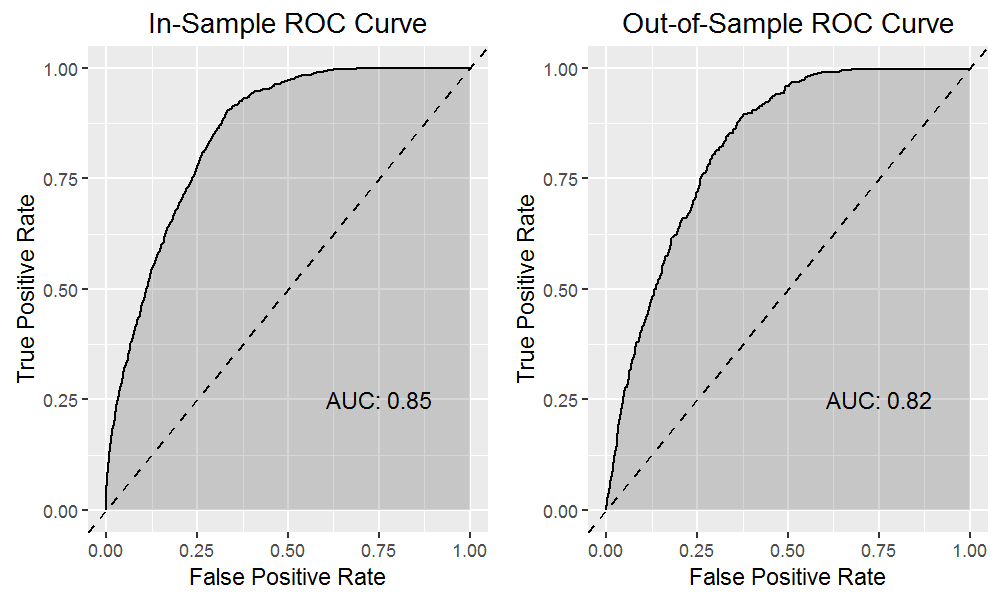
\includegraphics[height=2.60417in]{images/resp_m1_nb_sample_roc.png}

\paragraph{Figure A.2 ROC Curve: Random
Forest}\label{figure-a.2-roc-curve-random-forest}

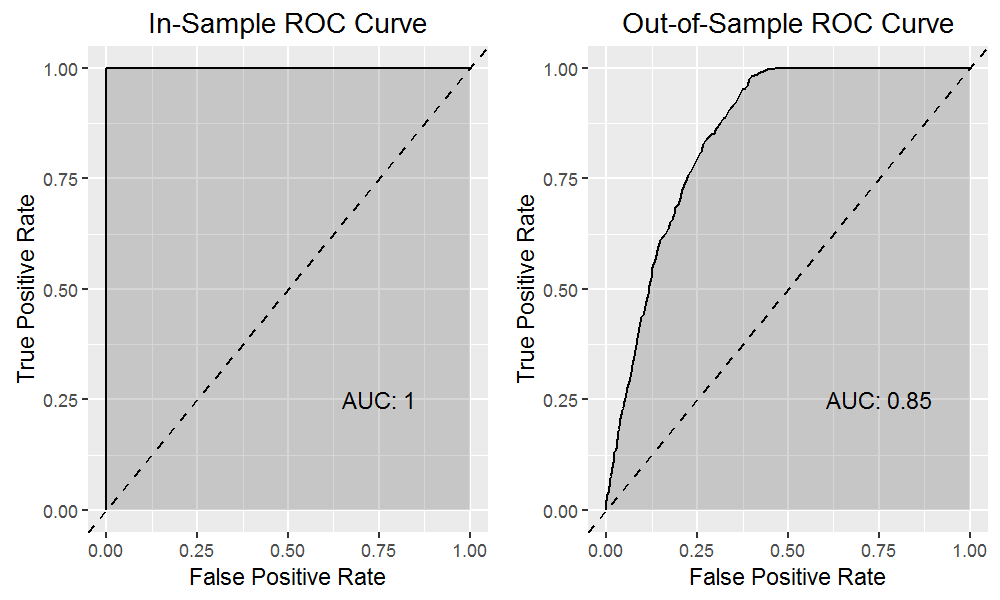
\includegraphics[height=2.60417in]{images/resp_m2_rf_sample_roc.png}

\paragraph{Figure A.3 ROC Curve:
GLMnet}\label{figure-a.3-roc-curve-glmnet}

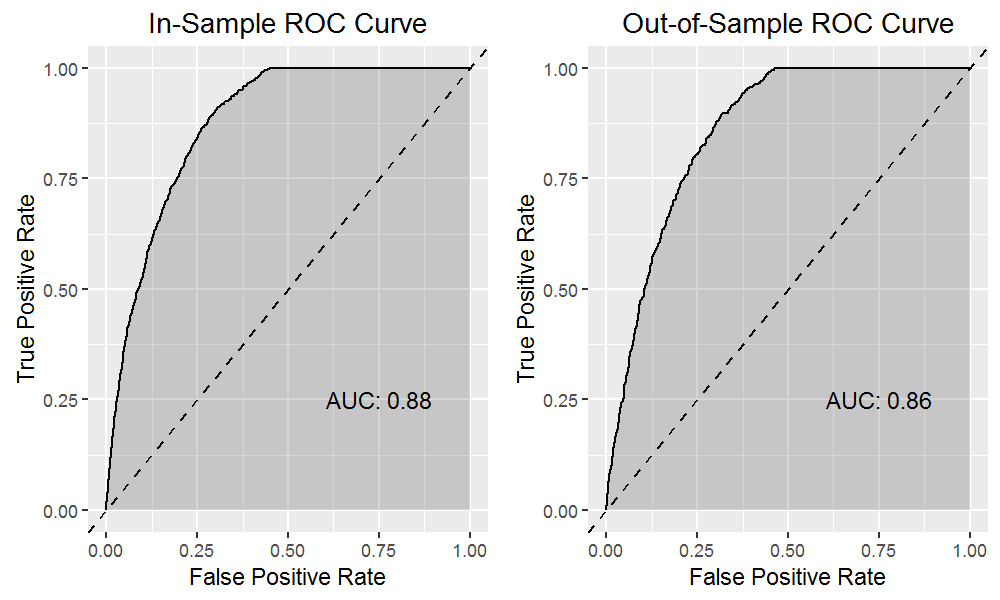
\includegraphics[height=2.60417in]{images/resp_m3_glm_sample_roc.png}

\newpage

\paragraph{Figure A.4 Actuals vs.~Predictions: Multiple Linear
Regression}\label{figure-a.4-actuals-vs.predictions-multiple-linear-regression}

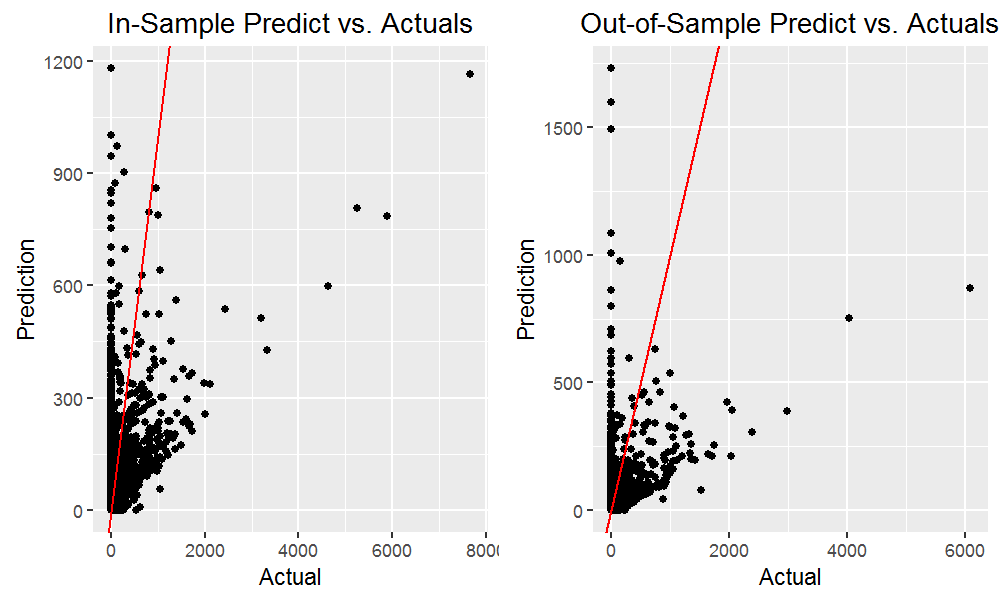
\includegraphics[height=2.60417in]{images/totamt_m1_lms_sample_pred.png}

\paragraph{Figure A.5 Actuals vs.~Predictions: Random
Forest}\label{figure-a.5-actuals-vs.predictions-random-forest}

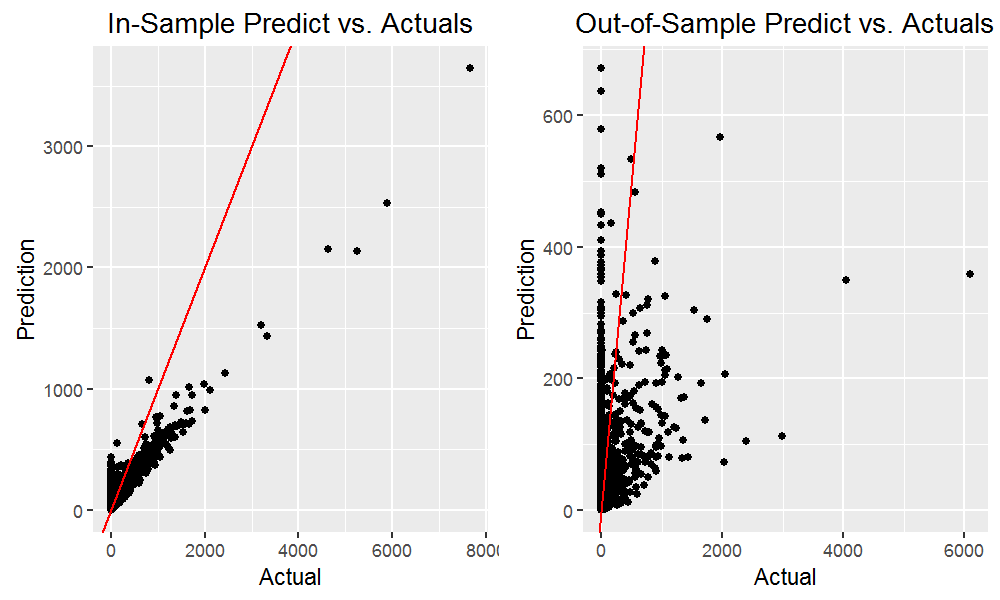
\includegraphics[height=2.60417in]{images/totamt_m2_rf_sample_pred.png}

\paragraph{Figure A.6 Actuals vs.~Predictions: eXtreme Gradient
Boost}\label{figure-a.6-actuals-vs.predictions-extreme-gradient-boost}

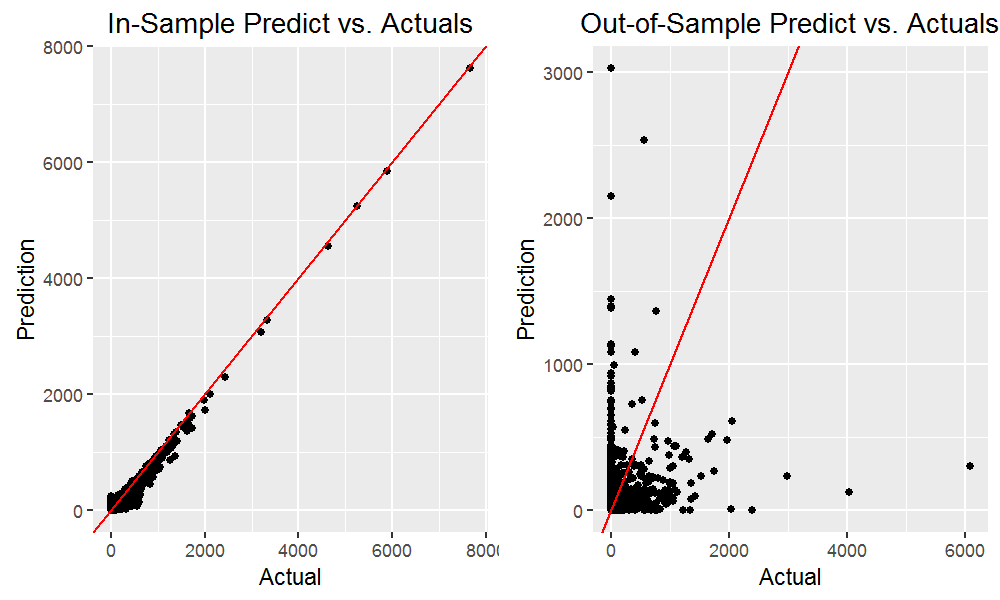
\includegraphics[height=2.60417in]{images/totamt_m3_xgb_sample_pred.png}


\end{document}
